\documentclass[a4paper]{article}
\usepackage[utf8]{inputenc}
\usepackage{graphicx}
\usepackage{siunitx}
\usepackage[version=4]{mhchem}
\usepackage{hyperref}
\usepackage{mathrsfs}
\usepackage{amssymb}
\usepackage{placeins}
\usepackage{wrapfig}


\title{Appunti di Chimica}
\author{Francesco Giuliano Rossi}
\date{A.A. 2025/2026}
\setlength\parindent{0pt}
\graphicspath{ {immagini} }
\hfuzz=10.0pt

\begin{document}
\maketitle
\tableofcontents
\newpage

\section{Atomo}
\subsection{Definizioni di Base}
Partiamo dal dare definizioni di basi 
\begin{enumerate}
    \item materiale - tutto ciò che ha massa e occupa spazio. 
    \item fasi - materia omogenea che in ogni suo parte può occupare tre stati:
    \begin{enumerate}
        \item solido - che ha un volume e forma propria
        \item liquido - che ha volume proprio e una forma data dal contenitore
        \item gas - privo di volume e forme propria
    \end{enumerate}
    \item molecole - costituiti da astomi, e possono essere 
        \begin{enumerate}
        \item omonucleare - molecole composti di atomi dello stesso elemento
        \item eteronucleari - molecole composte da atomi di diversi elementi
        \end{enumerate}
    \item elemento - una materia costituito da atomi di un solo tipo 
    \item composto - molecole eteronucleari
    \item miscele - materia composta da più composti/elementi. Possono essere
    \begin{enumerate}
        \item omogenee (si chiamano soluzioni), dove all'interno ci sono soluti che si trovano in concentrazione minore, e solventi che si trovano in concentrazioni maggiori
        \item eteronegee
        \item che hanno proprietá diverse in diversi punti
    \end{enumerate}
\end{enumerate}

\subsection{Atomi}
Per convenzione sono le unitá che costituiscono le sostanze. Le sostanze opssono essere costituiti da atomi di una solo specie atomica (sostanze elementari), o da specie di atomi diversi (composti). Le sostanze costituiscono la materia, e capire come sia fatto l'atomo è fondamentale per capire perchè la materie è fatta come la osserviamo. Questo è perchè cose uguali dal punto di vista chimico, possono essere uguali, ma poi non lo sono, come il petrolio e la plastica. 

L'atomo è costituito da protoni, neutroni, ed elettroni. Il raggio è dell'ordine di 1\AA (che è circa $\SI{10e-10}{m}$), mentre il nucleo ha un raggio di ~$\SI{10e-5}{\text{\AA}}$, quindi il nucleo in realtà contribuisce a poco del raggio dell`atomo totale. Il nucleo è composto da neutroni e potroni (e per questo si chiamano nucleoni, ovvero particelle che compongono il nucleo). Il neutrone non ha carica e la sua massa è $\SI{1.658e-27}{Kg}$, i protoni hanno una carica positiva di $\SI{1,6022e-19}{C}$ con una massa di $\SI{1,673e-27}{Kg}$ e gli elettroni ha carica uguale ma negativa al protone, con una massa di $\SI{9,1095e-31}{Kg}$. Alla fine gli elettroni contribuiscono poco alla massa della'tomo, ma contribuiscono tanto al volume. Quindi è principalmente il nucleo a dare il volume

\subsection{Nuclidi}
Un nuclide è un atomo caratterizzato dal numero atomico Z e numero di massa A. Il numero atomico ci dice quanti protoni ci sono nel nucleo mentre il numero di massa A da il numero di neutroni e protoni. Si scrive \ce{^{A}_{Z}Simbolo}. Il nuclide neutro ha un numero di elettroni uguali a quello di protoni. Per esempio l'elemento \ce{^{23}_{11}Na} ha 11 protoni, 11 elettroni, e 12 neutroni, mentre \ce{Na^+} ha meno solo 10 elettroni. Una carica positivo indica meno elettroni del normale, mentre un meno indica un elettrone in più. Cambiano solo il numero di elettroni perchè se cambiassero i protoni allora cambierebbe l'elemento. Se non è indicata una carica si assume che sia neutra. 

\subsection{Isotopi}
Nuclidi con lo stesso numero atomico ma con un numero di massa diversa si chiamano isotopi. Cambia il numero di protoni, e quindi cambia la massa, e c'è sempre uno più stabile degli altri (ogni elemento avrà una diversa distribuzione). Gli isotopi avranno proprietà chimiche e fisiche diverse dall'atomo originale. Molti isotopi non sono stabili, e nel complesso la dispersione degli isotopi cambia al variare nel tempo.

Conosciamo 120 specie atomiche, di cui 91 naturali, e 81 che hanno almeno un nuclide stabile. A bassi pesi atomici (Z$<$10), ad A=2Z si trovono molti elementi stabili. 

\subsection{Tavola Periodica}
La Tavola periodica degli elementi è ordinata per il numero atomico, dove le colonne (chiamati gruppi), hanno proprieà simili. Inoltre si chiama periodica perche` alcune proprietà si ripresentano in sequenza. Le colonne hanno proprietà chimiche molto simili, ma non uguali. Le proprietà chimiche dipendono interamente nel come gli elettroni si dispongono attorno il nucleo. I periodi, ovvero le righe avranno tutti numero quantico principale (chiamat iperiodi) uguali. Questa forma deriva dalla configurazione elettronica degli atomi all'aumentare del numero atomico.  
\begin{figure}[!h]
    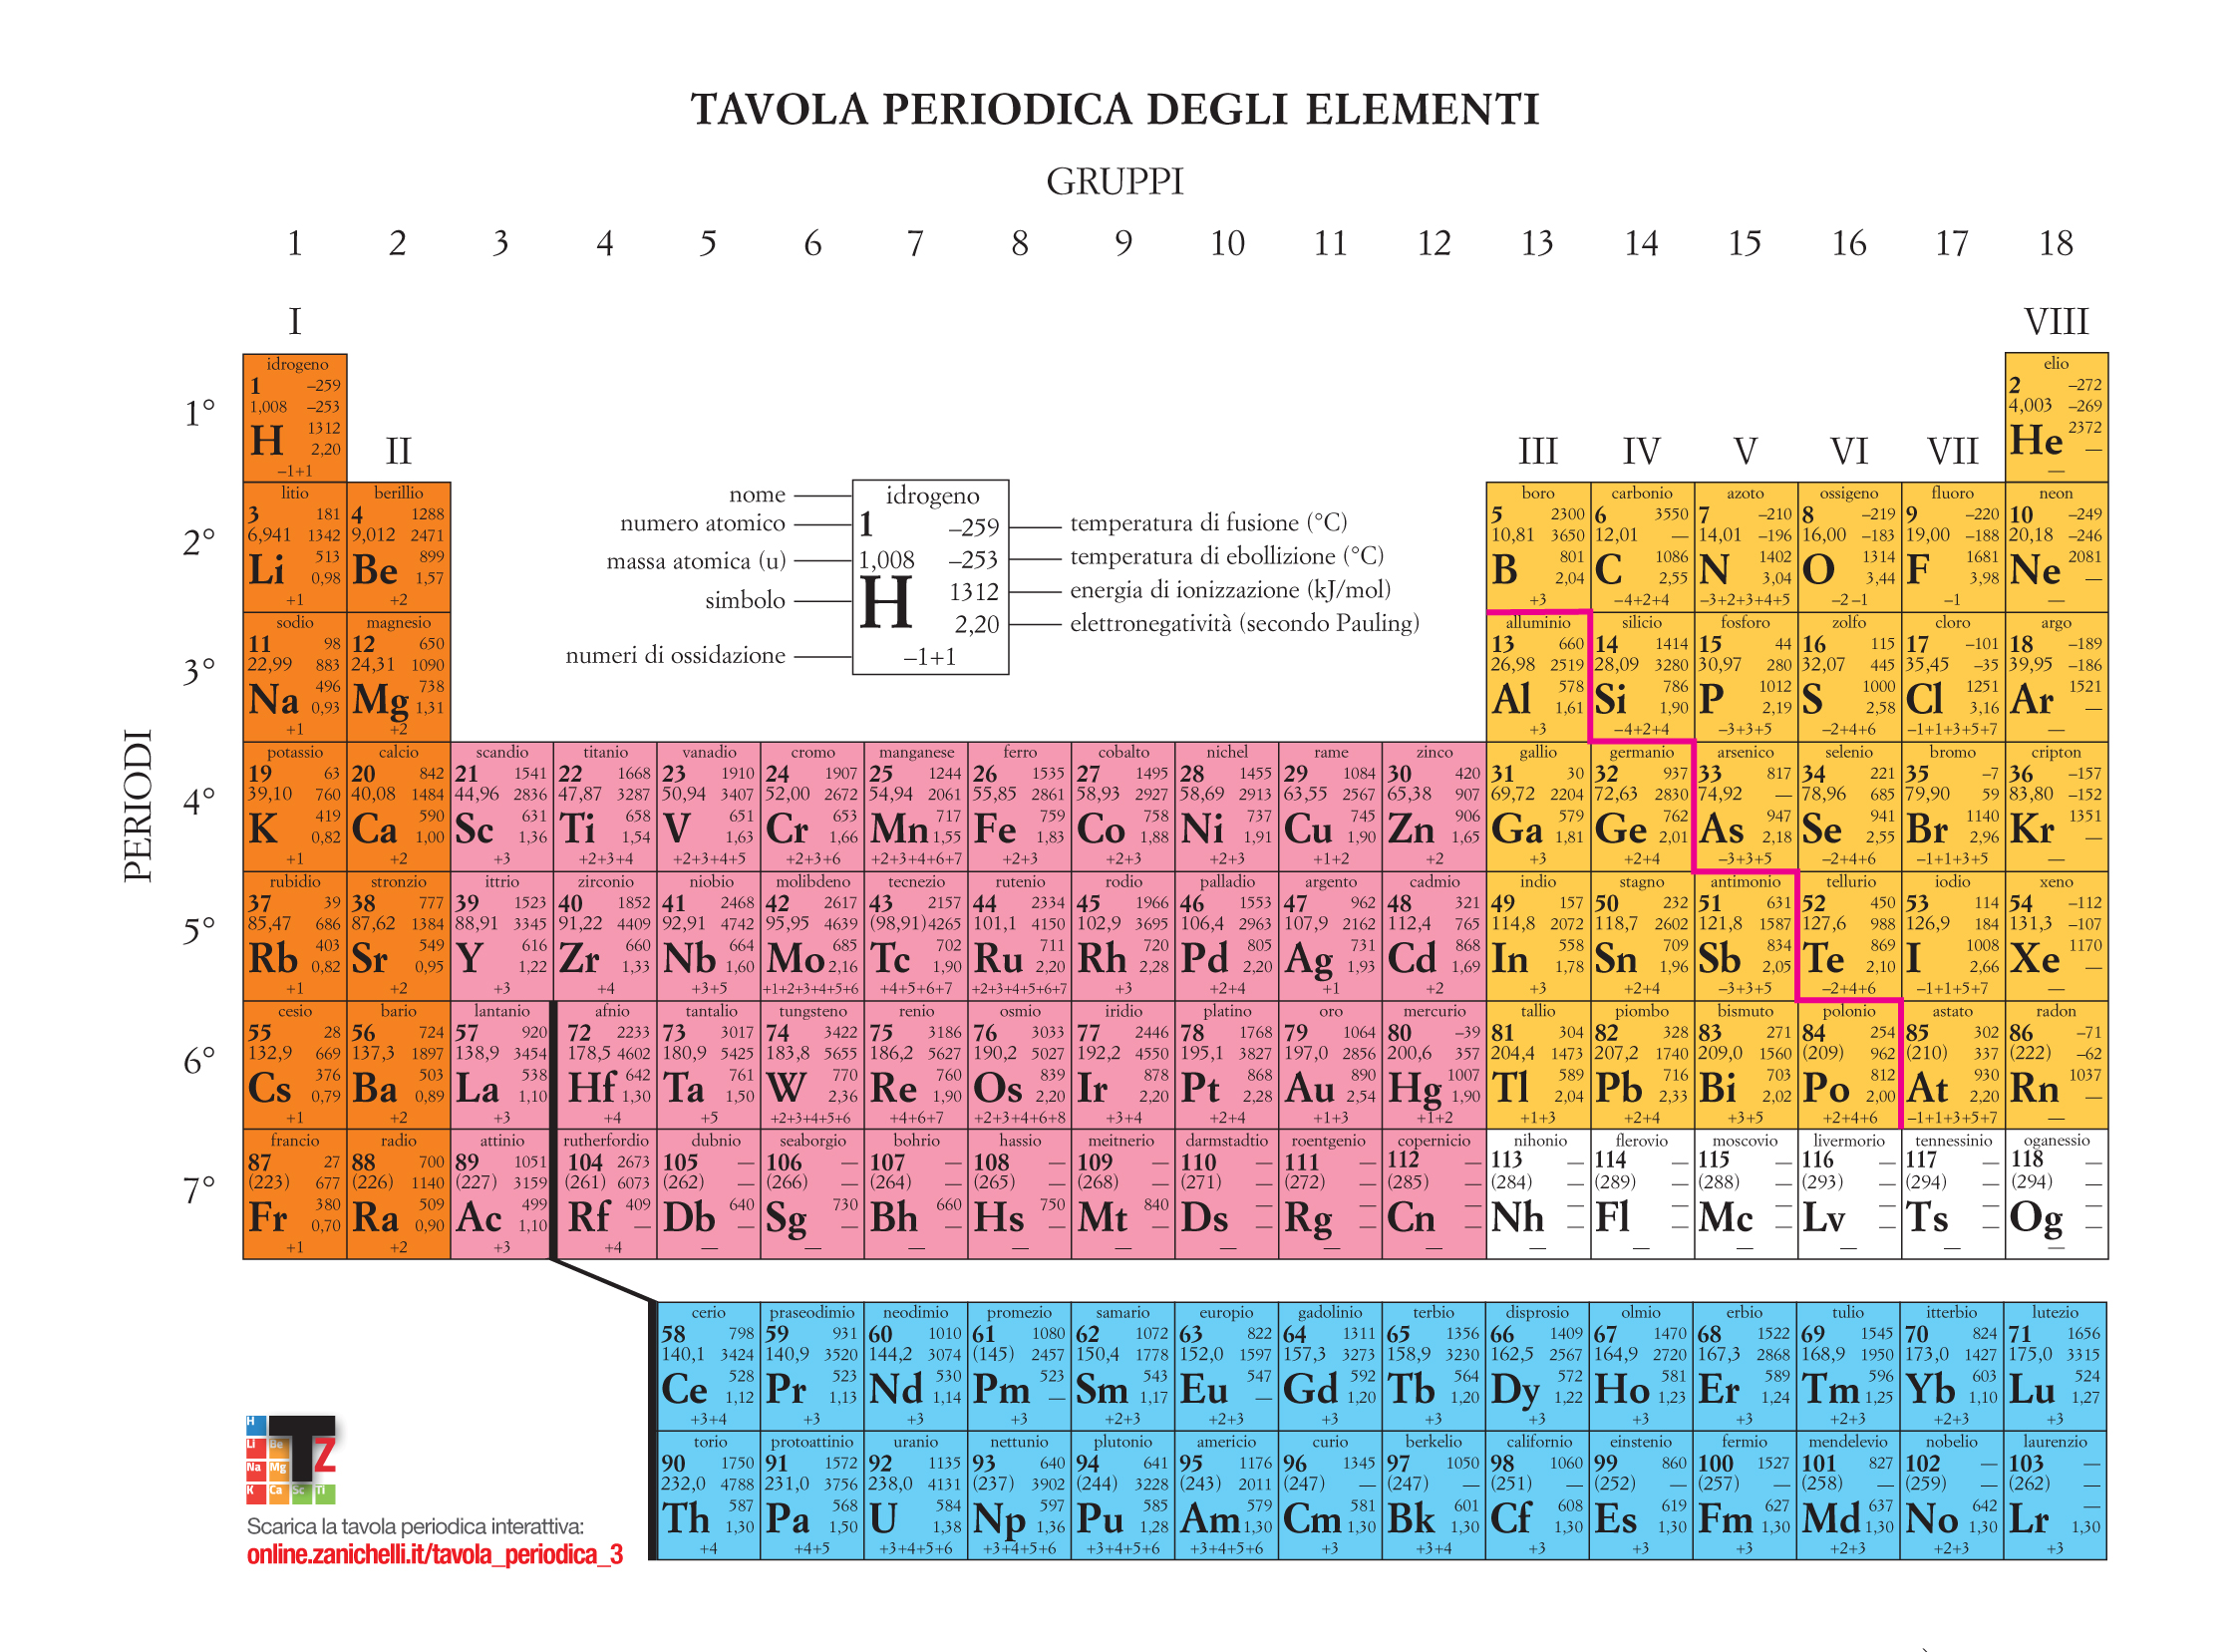
\includegraphics[width=\textwidth]{tavolaperiodica.jpg}
\end{figure}


\newpage
\subsection{Massa Atomica}
Stranamente, il valore sperimentale misurato della massa atomca è inferiore al valore ottenuto dalla somma delle masse di tutte le particelle sub-atomiche. Questo fenomeno si chiama \textbf{difetto di massa}, dove nella formazione del nucleo (costituito da legami tra nucleoni), si libera energia rispettando la legge E=mc$^2$. È di massimo 1\%, quindi l'elio \ce{^1_1H} non ha difetto massa, mentre \ce{^{238}_{92}Ur} subisce effetti grandi. 

L'unità di riferimento per la misura della massa degli atomi è uma (unità massa atomica), in inglese si chiama amu. Nel mondo biologico, è anche chiamata Dalton. È definita come $\frac{1}{12}$ della massa del nuclide neutro \ce{^{12}_6 C}. In questo modo abbiamo che un
\begin{itemize}
    \item Protone = \SI{1.007276}{uma}
    \item Neutrone = \SI{1.008665}{uma}
    \item Elettrone = \SI{0.0005486}{uma}
\end{itemize}

La massa Atomica relativa di un elemento è la media pesata rispetto all'abbondanza relativa degli isotopi naturali dei vari nuclidi neutri di un dato elemento. Per esempio, il Boro è costituito da \ce{^{10}_{}B} (massa $\SI{10.0129}{uma}$) al 19.91\% e da \ce{^{11}_{}B} (massa $\SI{11.0093}{uma}$) al 80.09\%. Allora la Massa Atomica Relativa risulta essere
\begin{equation*}
    M_B = 10.0129*\frac{19.91}{100}+11.0093*\frac{90.09}{100} = \SI{10.81}{uma}
\end{equation*}

Si può misurare la massa degli atomi sperimentalmente con lo spettrometro di massa. Viene messo sotto vuoto, e poi bombardato con elettroni che ionizzano gli atomi. Avviene all'interno di un condensatore elettrico, con tensione (allora positivi e negativi vengono separati). Vengono accelerati ed entrati in un elettromagnete, che cambia la traiettoria e il raggio di curvatura dipende dalla massa e velocità degli elettroni ed è inversamente proporzionale al campo magnetico e carica elettroni. Il campo magnetico è costante, anche la carica, allora dipende solo dalla massa. Preso tanti atomi diversi, il campione, ci saranno tutti gli isotopi che seguono una distribuzione. Per misurare la massa, si usa la massa atomica relativa. Vengono sempre cambiate perchè in natura avvengono continuamente reazioni nucleari a causa di fenomeni naturali. 

Se la massa atomica ha poche cifre significative, allora avrà tanti isotopi instabili, mentre se ha tante cifre significative, ha tanti isotopi stabili. Il \ce{^{2}_{1}H} si chiama Deuterio, mentre il \ce{^{3}_{1}H}, si chiama Trizio, ed è radioattivo. 


\subsection{Mole e Massa Molecolare}
La mole è un`unità molto importante in chimica. Misura la quantità di sostanza che contiene un Numero di Avogadro (N$_\text{A}$ $= \SI{6.022e23}{mol^{-1}}$) di entità elementari quali atomi, molecole, elettroni etc. Il numero di Avogadro viene definito come il numero di atomi presenti in 12 grammi di \ce{^{12}_{}C}.

Una molecola è cotituita da diversi atomi legati assieme, e la massa molecolare è la somma delle masse atomiche di tutti gli atomi che costiutiscono una molecola. Si definisce come \textbf{la massa di 1 mole di particelle}. Ha unità uma.

Per convertire da uma e grammi, abbaimo che \textbf{1 g = N$_A$ uma}


\subsection{Moderna Teoria Atomica}
\subsubsection{Equazioni di De Broglie}
La meccanica classica, anche se un ottimo modo per approssimare il comportamento di oggetti più grandi, al livello molecolare non funziona più. Per questo nasce la meccanica quantistica. La maggior parte di ciò che sappiamo è stato data dallo studio della luce emessa o assorbita. La radiozazione elettromagnetica trasporta energia nello spazio muovendosi ad una velocità di $\SI{3.00e8}{\frac{m}{s}}$. Anche se in fisaca classica le onde e corpi materiali sono diversi, nella meccanica quantistica sono la stessa cosa. Un'elettrone per esempio si può descrivere sia come particella, sia come onda. Questo dualismo si chiama la relazione di De Broglie, descritta dall'equazione 
\begin{equation*}
    \lambda = \frac{h}{mv}=\frac{h}{p}
\end{equation*}
dove $p=mv$ descrive il momento lineare della particella, h è la costante di Plank ($\SI{6.63e-32}{J s}$), e $\lambda$ è la lunghezza d'onda. Dato il valore della costante di Plank, i oggetti più grandi (scala umana), hanno una lunghezza d'onda talmente piccola che non possono essere misurati. Per esempio, la lunghezza d'onda  di un corpo di 1Kg che si muove 10Km/h è pari a $\SI{2.4e-32}{m}$. 

\subsubsection{Principio di Indeterminazione}
Un'altro concetto importante al livello della meccanica quantistica è il princcipio di indeterminazione. A grandezze classiche possiamo determinare due grandezze con qualsiasi grado di accuratezza, mentre nella meccanica quantistica non è vero. Il principio afferma che \textbf{non è possibile determinare contemporaneamente e con un'accuratezza arbitrariamente elevata alcune coppie di grandezze fisiche.} Ad esempio, per il momento p e la posizione di una particella lungo l'asse x, vale che 
\begin{equation*}
    \Delta p \cdot \Delta x \leq \frac{h}{4\pi}
\end{equation*}
Praticamente ci sta dicendo che se conosciamo l'energia accuratamente, allora l'incertezza sulla posizione sarà grande. Tante volte vorremmo precisione sull'energia, il che vuoldire che sacrifichiamo sulla precisione della posizione. 

\subsubsection{Equazione di Schrodinger}
In meccanica quantistica, uno stato di un sistema è completamente descritto dalla sua funzione d'onda o funzione di stato, che dipende dalle coordinate di tutte le particelle che costituiscono il sistema. Per un sistema quantistico possono esserci dinersi stati accessibili, ciascuno descritto da una funzione d'onda. Tutte queste si possono ricavare dall'equazione d'onda o equazione di Schrodinger. Dipende dalle coordinate spaziali, energia totale del sistema, e dalle interazioni tra particelle. L'equazione è 
\begin{equation*}
    H\Psi = E \Psi
\end{equation*}
dove H è l'operatore Hamiltoniano (??daphoque??), E è l'energia totale dell'elettrone descritto dalla funzione d'onda $\Psi$. Una funzione d'onda contiene la descrizione completa del sistema nello stato corrispondente, nel senso che tutte le caratteristiche fisiche del sistema in quello stato sono ricavabili da questa equazione. L'equazione ammette generalmente infinite soluzioni, ciascuno che descrive uno stato accessibile dal sistema. Ogni stato del sistema corrisponde una determinata energia totale. Questi stati si dicono \bfseries degeneri \mdseries se diversi stati corrispondono alla stessa energia. 

Un caso semplice è quando abbiamo un sistema costituito da una sola particella, in questo caso, il quadrato del modulo della funzione d'onda corrisponde ad un stato permesso $[\Psi(x,y,z)]^2$ ed è direttamente collegato alla probabilità che la particella si trovi nello spazio (questo è dato dalla quantità $[\Psi(x,y,z)]^2$ dV). Se questa particella si può spostare solo lungo l'asse x, entro uno spazio di dimensione L, l'equazione diventa 
\begin{equation*}
    -\frac{h^2}{8\pi^2m} \frac{d^2\Psi(x)}{d^2x}+V(x)\Psi(x) = E \Psi(x)
\end{equation*}
dove V(x) è l'energia potenziale della particella ed E è la sua energia totale. La funzione d'onda $\Psi$ descrive tutti gli stati accessibili al sistema che dipendono solo dalla variabile x. 
Le soluzioni sono 
\begin{equation*}
    E_n = \frac{n^2h^2}{8\pi L^2}
\end{equation*}
dove n è il numero quantico intero. Se n = 3, lo stato avrà 9 volte tanta energia quanto il primo stato. Inoltre, le n rappresentano quanti picchi (punti nodali) ci sono nell'onda. L può variare, e quando L diventa molto grande (nostro livello), le energie diventano così piccole che si possono trascurare. Ci si rende conto solo quando le distanze che consideriamo sono molto piccole. 

\subsubsection{Energia e Orbitali}
Il sistema più semplice è l'atomo di idrogeno, costituito da un protone e un elettrone (in realtà esiste anche $He^+$ che ha la stessa complessità). L'equazione d'onda per questo sistema può essere risolta esattamente, e quindi si può avere una formula analitica. Si trova che i valori di energia permessi sono dati da 
\begin{equation*}
    E_n = \frac{Z^2h \mathcal{R}}{n^2} \; \; \; \text{dove} \; \; \mathcal{R} = \frac{m_e e^4}{8h^3 \varepsilon_0^2}
\end{equation*} 
e dove n $\in \mathbb{N}$ è il numero quantico principale e risulta che l'energia di un sistema è quantizzata. Questo implica una serie di cose:
\begin{itemize}
    \item L'elettrone si può solo trovare in certi stati energetici
    \item Tutte le energie sono negative, l'elettrone possiede minore energia il più vicino è al nucleo
    \item All'aumentare di n, energie diventono meno negative
    \item Maggiore è la carica nucleare, più fortemente sarà legato l'elettrone al nucleo. Questa relazione è inversamente quadratica, quindi diventeranno sempre uno più vicino all'altro. 
\end{itemize}
Quando n=1 si dice che è uno stato fondamentale, mentre se n $>$ 1, si dice stato eccitato e l'elettrone passa da uno stato all'altro assorbendo o emettendo energia. Le funzioni $\Psi$ relative all'elettrone chiamate orbitali e descrivono le zone in cui si può trovare un elettrone in un atomo idrogenoide. Viene descritto dall'equazione 
\begin{gather*}
    \Psi(r,\theta,\phi) = R(r) \times Y(\theta, \phi) \\
    \text{funzione d'onda radiale} \; \; \; \; \; \text{funzione d'onda angolare}
\end{gather*}
Per descrivere un orbitale servono 3 numeri quantici: 
\begin{itemize}
    \item n: numero quantico principale (determina il guscio) e tutti gli orbitali con lo stesso valore hanno la stessa energia (detti degeneri)
    \item I: numero quantico di momento angolare orbitale (forma sottoguscio). Può andare da I = 0,1,...,n-1. Per I=0, orbitale S, I=1, orbitale p, I=2, orbitale d, I=3, orbitale f
    \item m$_I$: numero quantico magnetico, determina l'orientazione nello spazio, \\-I $\leq$ m$_I$ $\leq$ I
\end{itemize}
Un modo utile di rappresentare gli orbitali è di tracciare le superfici di contorno. È quella superfice in cui il valore della funzione è costante e tale che la probabilità di trovare l'elettrone nel volume racchiuso è più grande di un certo valore prefissato (90\%). Si trova calcolando 
\begin{gather*}
    \int_{V} |\psi(r,\theta,\phi)|^2dV = 0.9 \\
     \text{\small{(sostituisci 0.9 con la probabilità che vuoi)}}
\end{gather*}

La funzione di distribuzione radiale 
\begin{equation*}
    P(r)=r^2R^2(r)
\end{equation*}
rappresenta la probibiltà che un elettrone sia rinvenibile entro un guscio sottile di raggio r e spessore $\delta$r a presindere dalla direzione, mentre la funzione d'onda radiale rappresenta la probabilità di trovare un elettrone in un piccolo volume $\delta$V in una certa posizione dello spazio. Ci permette di fare una media di trovare l'elettrone su una superfice di spessore infinitesimo ad una distanza R. 
\begin{figure}[!ht]
    \centering
    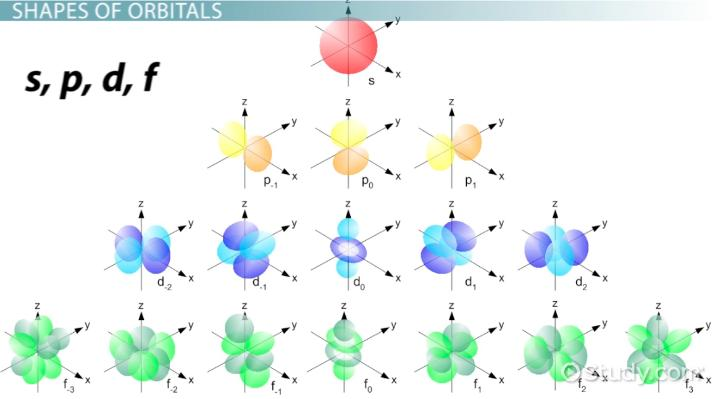
\includegraphics[width=0.65\textwidth]{orbitali.jpg}
    \caption{Vari Orbitali Possibili}
\end{figure}
\FloatBarrier

All'aumentare di n, aumenta il volume occupato da un orbitale, mentre all'aumentare di I diminuisce la probabilità di trovare un elettrone vicino al nucleo. Un orbitale esiste solo quando c'è dentro un elettrone. 

L'elettrone si può considerare come una sfera in rotazione sul suo asse e lo spin viene identificato con il numero quantico magnetico di spin m$_s$. Non ha nessuna relazione tra i numeri quantici, può solo assumere valori +1/2, o -1/2. Si chiama di spin perchè un elettrone porta con se un piccolo campo magnetico, che si genera come se l'elettrone stesse ruotando su se stesso. (anche se non si sa se effettivamente ruotano o no). 

\subsubsection{Come sono fatti gli orbitali?}
Gli orbitali S, non dipendono dalla parte angolare. La parte elettronica sarà concentrata in una sfera. Non dipenderà da $\theta$ e $\varphi$. Per il 2S, abbiamo uno zero (nodo), e per il 3S, abbiamo 2 nodi. L'1S, ha distribuizione continua, il 2S avrà superficie nodale, mentre 3S avrà 2 superfici nodali. 

Per gli orbitali P, hanno tutti la stessa forma, che sono palle simmetrici attorno gli assi cartesiani. Il piano definito dagli altri due assi è un piano nodale, in cui non si possono trovare elettroni. I colori diversi sono per ricordare che il segno della funzione d`onda è al contrario.

Gli orbitali D, 4 hanno 4 nodi, con due piani nodali, che stanno distesi nei piani xy, yz, xz, mentre il quinto ($z^2$), composto di due nodi, è un toroide. 

Orbitali f hanno o 6 o 8 nodi. Complicato, guarda disegno. 

All'aumentare n, aumenta il volume occupato da un orbitale. Gli orbitali avranno sempre la stessa forma, ma il volume che occupa è molto più grande, non importa quanti superfici nodali ci sono dentro. All'aumentare di l (quindi cambia lettera), diminuisce la probabilità di trovare un elettrone vicino al nucleo. Quindi quando ci mettiamo più di un elettrone avrà un effetto molto grande. 

\subsubsection{Gli atomi polielettronic}
Le soluzioni dell'equazione d'onda per un atomo costituito da un nucleo ed N elettroni sono delle funzioni di 3N variabili. Un'approssimazione molto usata per trovare una soluzione è l'approssimazione orbitalica, dove il nucleo viene considerato immobile, e la funizone d'onda viene scritta come una combinazione di orbitali monoelettronici (come idrogenoide). In questo modo, la funzione d'onda ottenuta ci permette di stabilire la configurazione elettronica di un atomo. 

Si può dire che la configurazione elettronica di un atomo è l'elenco di tutti gli orbitali occupati dagli elettroni di quell'atomo. Diversamente dagli atomi idregenoidi, l'energia degli orbitali non dipende solo da n (numero qauntico principale), ma anche da I (numero quantico momento angolare). Questo vuoldire che un elettrone descritto da orbitale 2s sarà diverso da uno descritto da 2p e viene chiamato l'effetto schermo. Per questo la struttura di un atomo polielettronico viene descritto in termini di strati o gusci elettronici. Lo strato elettronico più esterno viene detto strato di valenza. 

\subsubsection{Effetto Schermo}
Un guscio elettronico non percepisce solo l'attrazione della carica nucleare, ma anche la repulsione dei gusci elettronici più interni (electron in 3rd layer is forced away by electron in 2nd layer). La carica risultante si chiama carica nucleare efficace, Z$_{eff}$. La carica nucleare efficaie varia al variare del numero quantico momento angolare I. Visto che l'elettrone descritto da una funzione d'onda di tipo s riesce ad essere più vicino all'elettrone di tipo p con lo stesso n, l'effetto schermo sull'elettrone s, sarà minore di quello sull'elettrone p. 
\begin{figure}[!ht]
    \centering
    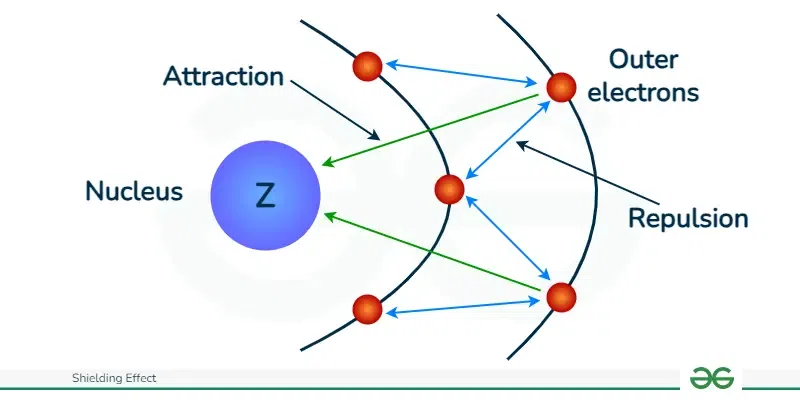
\includegraphics[width=0.75\textwidth]{Shielding-Effect.jpg}
    \caption{Shielding Effect (effetto schermo)}
\end{figure}
\FloatBarrier
Lo stesso ragionamento vale per elettroni p e d (con stesso n), e così via. L'ordine segue s $>$ p $>$ d $>$ f $>$ ...  

\subsubsection{Più orbitali}
Nel passare dall'atomo di idrogeno ad un sistema polielettronico, l'aumento della carica nucleare provoca un abbassamento dell'energia di tutti gli orbitali. \\
\begin{center}
    \textbf{\Large{Trucchetto per ricordare!!!}}
\end{center}
A causa dell'aumento dell'energia degli orbitali all'aumentare di l, orbitali con un certo ned un elevato numero quantico angolare possono avere più energia di un orbitale con un numero quantico angolare basso e numero quantico principale (n+1) maggiore. A causa dell'effetto schermo, questo ordine può essere invertito. In generale, per questa classe di atomi, l'energia degli orbitali è data da n+l, e a parità di questo valore, dal valore di n. Energia non dipende da n+l. 

Occhio che si deve anche guardare la parte analitica, ovvero le formule, e vanno moltiplicate quelli giusti di funzioni d'onda radiali e angolari. Quella radiale va a zero per la distanza che aumenta. Prima della parte radiale c'è sempre un polinomio, che ha valore 0 per l=0, e quindi non dipende da R, ma è una costante. Puoi solo moltiplicare parti radiali e angolari che hanno lo stesso n. Tutti gli altri orbitali si posso scrivere come combinazione lineare degli orbitali angolari e radiali. 

\subsubsection{Principio di esclusione di Pauli}
Il principio di esclusione di Pauli afferma che un orbitale non può essere occupato da più di due elettroni e, se questi occupano lo stesso orbitale, i loro spin devono appaiarsi. Due elettroni quindi non possono essere descritti dalla stessa quaterna di numeri quantici. 

\subsubsection{Principio di Aufbau}
Questo ci da una regola per la costruzione della configurazione elettronica. Gli elettroni si associano a partire dall'orbitale disponibile a minor energia, senza mai superare il numero di 2 elettroni per orbitale. Inoltre, la regola di Hund dice che la configurazione più stabile è quella caratterizzata dal maggior numero possibile di elettroni spaiati con spin parallelo. Vogliamo che tutti gli elettroni hanno lo spin nello stesso verso. Dal Carbonio in poi, dobbiamo usare il Principio di Aufbau, come segue in figura
\begin{figure}[!ht]
    \centering
    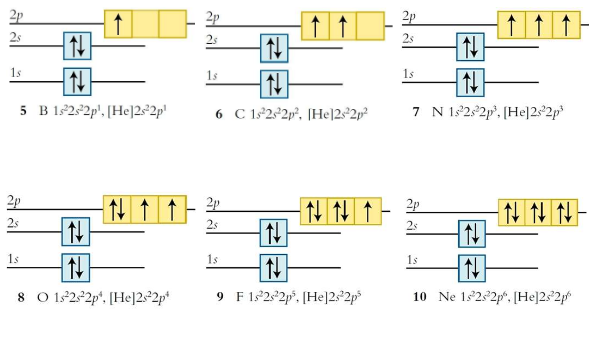
\includegraphics[width=0.75\textwidth]{orbitali.png}
    \caption{Orbitali di elementi più pesanti}
\end{figure}
\FloatBarrier
La configurazione del Neon è detto configurazione guscio chiuso, perchè ogni orbitale contiene una coppia di elettroni. Quelli dell'azzoto è detto semichiuso perchè ogni orbitale contiene singolo elettrone. Dovrò inserire quanti elettroni quanti elettroni dell'elemento chimico che ci interessa.

\subsection{Elementi diamagneici e paramagneitici}
Non sempre sono seguiti le regole perfettamente. 

Per esempio con il cromo \ce{^{52}_{24}Cr}. La configurazione elettronica è 3d$^5$4s$^1$ (quindi tutti gli orbitali sono riempiti), e non 3d$^4$4s$^2$ (dove abbiamo orbitale 4s che è pieno e 3d che non lo è). La differenza di energia è relativamente piccola, e l'atomo lo fa solo in caso che gli conviene, se si trova in questo primo stato, poi avrà tutti gli semigusci pieni, e tutti gli orbitali saranno occupati da atomi con spin parallelo. Avrà sottogusci semioccupati, e quindi si avrà un sistema più stabile. L'energia potenziale dell'atomo diminuisce con 3d$^5$4s$^1$. 

Stessa cosa succede con tutti gli atomi che hanno 5 elettroni in più, e che stanno sotto il rame. 

Con lo scandio (Scandium \ce{^{44.96}_{21}}Sc), l'orbitale 4s viene completato e gli orbitali a più bassa energia disponibili sono i cinque 3d che possono avere 10 elettroni e si ha così la prime serie di metalli di transizione. In realtà la differenza di energia tra livelli 4s e 3d è molto piccola. Se la configurazione prevede almeno un elettrone spaiato, si chiamano elementi paramagnetici, se no si chiamano diamagnetici. Quelli paramagnetici vengono attratti dal campo magnetico, quelli diamagnetici debolmente rispinti. 

\subsection{Elettroni di Valenza ed Interni}
Gli elettroni contenuti nel guscio elettronico più esterno si chiamano elettroni di valenza. Quelli all'interno del guscio di valenza si chiamano elettroni interni. Quelli di valenza sono quelli che hanno più energia, più lontani dal nucleo, e quindi sono quelli che entrano in gioco durante reazioni chimiche. Se consideriamo $1s^22s^22p^63s^23p^63d^54s^1$, solo $3d^54s^1$ sono elettroni di valenza, e si abbrieva gli elettroni interni scrivendoli come elementi, quindi questa sequenza si scriverebbe [Ne] $3d^54s^1$. Quelli interni non avranno molto effetto durante le reazioni chimiche. 

Nella tavola periodica esistono 4 blocchi, tutti chiamati s, f, d, p, che rappresentano l'ultimo orbitale riempito. Per questo anche la tavola periodica ha la forma che ha, perchè si basa sugli orbitali e vengono ordinati in energia crescente. 

\begin{figure}[!ht]
    \centering
    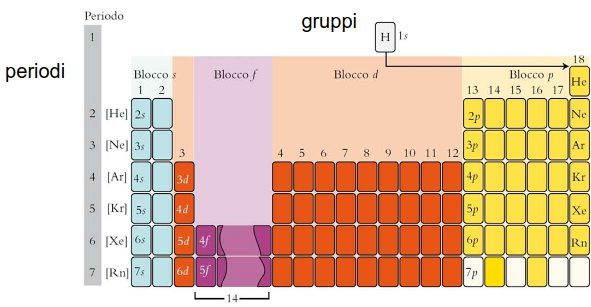
\includegraphics[width=\textwidth]{tavolaperiodicablocchi.png}
    \caption{Tavola periodica divisi in blocchi}
\end{figure}
\FloatBarrier

Tutti gli elementi vogliono avere gusci chiusi, perchè è la configurazione più stabile. Infatti, quando voglio rompere il guscio completo più esterno mi serve tanta energia per farlo. 

\subsection{Proprietà periodiche}
Le proprietá periodiche dipendono da come la carica nucleare efficacie cambia lungo il periodo e lungo il gruppo. Questo succede per i primi 18 elementi chimici (prima dell'orbitale p). L'idrogeno è l'unico 'pulito' che ha un $\mathbb{Z}_{eff}$ intero. L'effetto schermo non è del tutto lineare, ma per la maggiorprte si. Arrivato al 2p, si arriva al $3s^1$, e $\mathbb{Z}_{eff}$ cala abbastanza, perhcè il prossimo elemento avrà 10 elettroni che gli fanno da schermo per la carica nucleare. Poi passato al 3p, avrà un $\mathbb{Z}_{eff}$ lineare, e questo si ripete abbastanza periodicamente (hahahha).

\subsubsection{Raggio Atomico}
Come si definisce il raggio dell'atomo? Visto che gli elettroni sono descritti da funzioni d'onda che si estendono in teorea all'infinito, non è un concetto banale. 

Solo i gas nobili si possono individuare in uno stato monoatomico. Definirlo per un gas nobile ha senso, ma se non si presenta in una forma monoatomica in natura non ha senso definirlo. Per questi che non ha senso definilri in forma monoatomica, li definiamo usando le moleole biatomiche omonucleari.

Per molecole biatomiche omonucleari gassose, si può determinare sperimentalmente la distanza tra i due nuclei, considerando le sfere tangenti, e il raggio viene preso come la metà di questa distanza. Questi possono poi essere usati per determinare il raggio di altri elementi. Il più a destra che si va nella tavola periodica il raggio diminuisce, il più basso, il più aumenta (diminuisce lungo un periodo e aumenta secondo in un gruppo).

Si osserva che spostandosi da sinistra verso destra si aggiungono protoni ed elettroni allora i protoni aggiuntivi determinano un aumento della carica nucleare, ma i elettroni non operano un effetto scherma così efficace come quello realizzato dagli elettroni degli strati interni. Questo poi implica che la carica nucleare efficace aumenta e allora la dimensione atomica diventa più piccola.

Scendendo lungo un gruppo la configurazione atomica rimane la stessa a parte un incremento del numero quantico principale n. Questo incremento comporta una maggior distanza media degli elettroni dal nucleo e tale distanza non viene compensata dalla carica nucleare, risultando in un espansione del volume atomico. \\

tldr: diminuisce lungo periodo, aumenta lungo gruppo. 

\subsubsection{Raggio Ionico}
In base all'andamento del raggio ionico si può vedere eche diminuisce lungo un periodo e aumenta scendendo in un gruppo. La motivazione è lo stesso per il raggio atomico. Va osservato che i cationi (ione carico positivo) hanno un raggio molto più piccolo degli atomi neutri di partenza mentre per gli anioni (ioni carico negativamente) hanno raggio molto più grande. Attento a i isotopi, che possono avere stesso layout elettronico di un altro elemento. 

\subsubsection{Energia di Ionizzazione}
L'energia di ionizzazione è la variazione di energia necessaria per espelere un elettrone da un atomo isolato (atomo non è legato a nessun altro tipo di atomo, non forma nessuna molecola) allo stato gassoso (g) (perchè gli atomi staranno molto lontani e quindi la frequenza con cui si sbattono è molto minore). 
\begin{gather*}
    x(g[assoso]) \rightarrow X^+(g)+e^-\\
    \Delta E = \text{Energia del sistema}(X^+(g)+e^-) - \text{Energia del sistema} (X(g))
\end{gather*}
Se $\Delta E > 0$ allora lo stato finale ha energia più elevata dello stato iniziale e si parla di un processo energeticamente sfavorito. Se $\Delta E<0$ allora lo stato finale ha energia minore (e più stabile) dello stato iniziale e il processo si definisce energeticamente favorito. All'opposto del raggio atomico, il più che si va a destra nella tavola periodica, la quantità aumenta, mentre il più che si scende diminuisce. Questo si basa sempre sull'aumento della carica nucleare efficace, che lega più fortemente gli elettroni aggiunti e quindi richiede più energia per espellere uno. Scendendo lungo un gruppo, l'elettrone espulso è descritto da un numero quantico principale sempre maggiore e allora si trova più lontano dal nucleo e sente più effetto di schermatura. 

L'energia di ionizzazione monoatomico è diverso da quello biatomica. Non basta avere solo monoatomica, deve proprio essere isolato

Quando un elettrone non è più legato, si chiama fotoelettrone. Servono per misurare l'energia di legame all'interno dell'atomo. L'energia che serve per espellerla si chiama binding energy. Questa energia è fortemente legata all'intorno dell'atomo. 

Si possono definire più energie di ionizzazione, l'energia della prima ionizzazione (I$_1$) si riferisce ad un ione monopositivo (carica +1), e l'energia di seconda ionizzazione I$_2$ che si riferisce alla formazione di ione carica +2, etc. Questa energia, generalmente aumenta. Da notare che serve meno energia per espellere un elettrone del guscio di valenza a quella di un elettrone interno. Cambia ovviamente se per ionizzarlo devo togliere un elettrone da un guscio. Per questo può aumentare di tanto l'energia di prima ionizzazione necessaria. Come nel caso del \ce{^{6.941}_{3}Li}

Tipo in caso del Boro, parto da 
\begin{gather*}
    1s^22s^22p^1 \rightarrow 1s^22s^2 \rightarrow 1s^22s^1 \rightarrow 1s^2 \\
    poca \; \; \; \; tanta \; \; \; \; poca \; \; \; \; tanta
\end{gather*}

tldr: aumenta lungo periodo, diminuisce lungo gruppo


\subsubsection{Affinità elettronica}
Questa è la variazione di energi, cambiato di segno, che si ha quando un atomo neutro isolato gassoso acquista un elettrone diventando un ione negativo:
\begin{gather*}
    X(g)+e^- \rightarrow X^-(g) \\
    \Delta E = \text{Energia del sistema}(X^-(g)) - \text{Energia del sistema}(X(g)+e^-)
\end{gather*}
In questo modo un grande valore di affinità elettronica vuoldire un valore molto negativo in $\Delta E$. Se ha un alta affinità eletttronica, l'acquisizione di un elettrone è p` alto (un processo che è energeticamente favorito). Se ha un basso valore di affinità elettronica allora l'elemento ha scarsa tendenza ad acquistare un elettrone in più. All'andare a sinistra nella tavola periodica aumenta l'affinità elettronica (dato dall'aumento della carica nucleare efficace), mentre sulle colonne c'è poca variazione (più difficile da spiegare). Anche qua dipende dal cosa succede alla molecola dopo che viene aggiunta un elettrone. Può comportarsi come un gas nobile, e quindi ci vuole energia per aggiungerli elettroni. 

Tra il livello 14 e 15, c'è un saltino perché dipende dal isstema di partenza e finale. Per il carbonio, l'affinità elettronica è molto favorito perchè poi arriva alla configurazione $Np^3$, con un semiguscio chiuso. Questo è una situazione molto stabile. Mentre per l'azzoto questo è meno positivo perchè da una configurazione stabile si va a creare una più instabile. Si aggiunge un $Np^4$, e quindi cambia configurazione. 

\subsubsection{Elettronegatività}
Questo è la tendenza di un atomo ad attrarre verso di se gli elettroni durante una reazione chimica. Si indica con $\chi$. Tutti i valori si possono ricavare da quello dell'energia di ionizzazione e affinità elettronica. Aumenta da sinistra verso destra e diminuisce alto verso basso. 
\begin{equation*}
    \chi = \{D(A-B)-\frac{1}{2}[D(A-A)-D(B-B)]\}^{\frac{1}{2}}
\end{equation*}
\textbf{aggiungere perchè si comporta in questo modo}

\section{Formazione di uno Ione}
Un atomo isolato è neutro perchè ha il numero di elettroni uguali al numero di protone. Quando un atomo viene a contatto con un altro atomo per formare un legame o molecola, spesso la sua elettroneutralità viene perturbata. Può cedere uno o più elettroni, trasformandosi in un ione (positivo o negativo). Messi più ioni insieme si chiamano composti ionici. Un esempio è NaCl, costituito da Na$^+$ e Cl$^-$. 

\subsection{Ioni}
Gli ioni possono essere monoatomici o poliatomici (gruppi di atomi), che portano una carica elettrica. Viene sempre indicata a destra in apice rispetto alla formula chimica dello ione. Se ci sono più elettroni si scrive n$\pm$. 

Esistono gruppi che generano ioni in maniera ben precisa. Tutti quelli che stanno a sinistra (1o 2o gruppo), generano tutti cationi (perdono elettroni), perchè così acquisiscono la configurazione del gas nobile che precede il numero atomico. Quelli del primo primo (metalli alcalini), sono metalli che generano ioni con carica +1. Quelli del secondo gruppo (alcalino terrosi), e sono metalli che generano ioni con carica +2. Non esiste lo ione C$^+$. Allo stesso modo quelli del grupo 13 perdono 3 elettroni e quindi avranno carcica +3. 

\begin{wrapfigure}{l}{0.35\textwidth}
    \begin{center}
    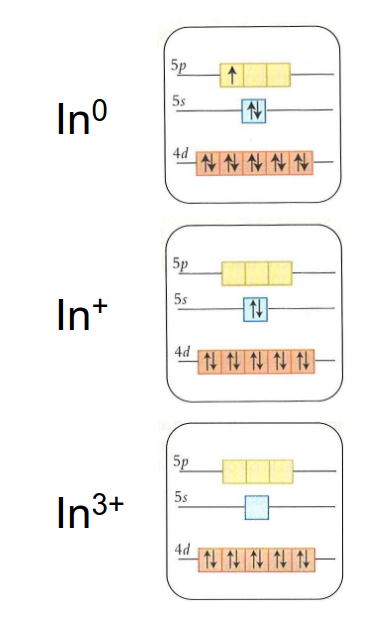
\includegraphics[width=0.35\textwidth]{indio_ione.png}
    \end{center}
\end{wrapfigure}
\FloatBarrier

Alcuni metalli del blocco p, con un numero quantico principale più alto possono generare 2 tipi di elettroni. Tipo per l'indio, si possono avere questi ioni. 

Quelli degli ultimi gruppi hanno la tendenza di acquistare elettroni in più, per trasformarsi in anioni per arrivare ai gas nobili che sono dopo. Tipo il Cloro acquista 1 elettrone per arrivare ad avere la configurazione elettronica dell'Argon. 

\subsection{Stato di Ossidazione}
Lo stato di ossidazione è il numero di atomi che cederebbe o guadagnerebbe quando forma un legame chimico. Si possono prevedere sulla base della configurazione elettronica dell'elemento neutro. Sono generalmente pochi per ogni elemento chimico. \\

Esempio: Tipo il Selenio \ce{^{}_{34}Se} ha $1s^22s^22p^63s^2$ $3p^64s^23d^{10}4p^4$ e questo 4p$^4$, ha 2 elettroni che mancano per completare il guscio. Quindi dovrebbe guadagnare due cariche diventando Se$^{2-}$ (orbitale 4p$^6$, per avere il guscio pieno. Si potrebbe anche avere il Se$^{4+}$ (orbitale $4s^23d^{10}$), o anche il Se$^{6+}$ (orbitale 3d$^10$), ma quest'ultimo è più difficile avere. Gli ultimi due hanno una carica così grande che non si troveranno mai da soli. 

Inoltre, esiste anche un'altro stato, ovvero il Se$^0$, ovvero quello neutro, che è certo per ogni elemento chimico. Se$^{2-}$ esiste anche da solo, come in CdSe e PbSe (questi due si trovano nei QD-LED display). 

\subsection{Numero di Ossidazione}
La maggiorparte dei composti non sono ionici, ma quando due atomi diversi sono legati, uno dei due tende ad attirare gli elettroni dell'altro verso il proprio nucleo. Se uno è più elettronegativo dell'altro atomo, non saranno equalmente distribuiti in un legame chimico. Se uno è molto elettronegativo e l'altro poco, uno perde l'elettrone e si crea un legame ionico. Per un modo semplice di come si distribuiscono nei atomi, si introduce il numero di ossidazione. È un numero fittizzio, che ha poco a che fare con la carica dell'atomo. 

È definito come la carica che un dato atomo assumerebbe in un composto se tutti i legami che lo coinvolgono fossero completamente ionico. Tutti gli elettroni vanno assegnati agli atomi più elettronegativi. Serve solo per capire quale elemento tende a prendere più elettroni e quali tendono di più a cederli. 

Siccome un atomo isolato è neutro, numero di ossidazione è 0. In una qualsiasi molecola omonucleare non ci possono essere differenze in come si attraggono gli elettroni visto che sono tutti lo stesso elemento. Quando invece abbiamo uno ione monotomico, come Na$^+$, il numero di ossidazione corrisponde alla carica netto dello ione (+1 in questo caso).

Alcune regole 
\begin{enumerate}
    \item l'idrogeno forma sempre solo un legame $\rightarrow$ avrà un numero di ossidazione sempre +1 quando è legato ad elemento con elettronegatività più alta e -1 quando è meno. 
    \item il fluoro forma sempre un legame singolo, sarà sempre -1 (perchè è più elettronegativo)
    \item Per soddisfare regola dell'l'ottetto l'ossigeno tende a formare sempre due legami. \begin{enumerate}
        \item Siccome solo il fluoro è più elettronegativo, in un composto, l'ossigeno avrà quasi sempre -2. OF$_2$, ossigeno è +2
        \item Con i perossidi, fatto tra 2 atomi di Ossigeno legati fra loro e legati ad altri elementi meno elettronegativi. Il legame che lega i due ossigeni, sarà pari, allora l'ossigeno avrà numero di ossidazione -1. 
    \end{enumerate}
\end{enumerate}

La somma algebrica di numeri di ossidazione degli elementi costituenti una data specie chimica deve essere ugual ealla carica netta della specie stessa. Se hanno un numero di ossidazione uguale, vuoldire che hanno proprietà chimiche molto simili. 

\end{document}